\section{Smalltiles}
Este filtro consiste en replicar 4 veces la imagen original achicada. De esta manera, si enumeramos los píxeles a partir del 0, siempre estaremos utiplizando los píxeles de número par de la imagen original para generar las 4 más pequeñas.
\subsection{Código C}
	En el código de C recorremos el equivalente a una de las 4 fotos pequeñas. En el píxel de la posición \emph{(i,j)} guardamos el contenido del de la posición \emph{(2*i,2*j)} en la imagen original. A la vez cargamos este contenido en las otras 3 imagenes.
	A continuación mostramos el pseudocódigo de Smalltiles:
\begin{algorithm}[h!]
\caption{Smalltiles}
\begin{algorithmic}
  \Function{smalltiles}{src: *unsigned char, dst: *unsigned char, cols: int, filas: int, srcRowSize: int, dstRowSize: int}
	\State $unsigned~ char~ (*srcMatrix)[srcRowSize] = (unsigned~ char (*)[srcRowSize])~ src$
	\State $unsigned~ char~ (*dstMatrix)[dstRowSize] = (unsigned~ char (*)[dstRowSize])~ dst$
	\State int ancho $\gets$ col/2
	\State int largo $\gets$ filas/2
	\For{$f \gets 0~..~largo-1$}
		\For{$c \gets 0~..~ancho-1$}
			\State $bgra_t* p_s \gets (bgra_t*)$ \& $srcMatrix[f][c * 4]$
			\For{$i \gets 0~..~1$}		
				
				\State $bgra_t *p_d \gets (bgra_t*)$ \&$dstMatrix[f][(c + ancho*i) * 4]$
				
				\State ($p_d \rightarrow$b) $\gets$ ($p_s \rightarrow b$)
				\State ($p_d \rightarrow$g) $\gets$ ($p_s \rightarrow g$)
				\State ($p_d \rightarrow$r) $\gets$ ($p_s \rightarrow r$)
				\State ($p_d \rightarrow$ a) $\gets$ ($p_s \rightarrow a$)
			\EndFor
			\For{$i \gets 0~..~1$}		
				
				\State $bgra_t *p_d \gets (bgra_t*)$ \&$dstMatrix[f + largo][c * 4]$
				
				\State ($p_d \rightarrow$b) $\gets$ ($p_s \rightarrow b$)
				\State ($p_d \rightarrow$g) $\gets$ ($p_s \rightarrow g$)
				\State ($p_d \rightarrow$r) $\gets$ ($p_s \rightarrow r$)
				\State ($p_d \rightarrow$ a) $\gets$ ($p_s \rightarrow a$)
			\EndFor
		\EndFor
	\EndFor
\EndFunction

\end{algorithmic} 
\end{algorithm}
	
\subsection{Código ASM}
	
	
	
\subsection{Experimentación}

\subsubsection{Idea}
Nuestra implementación de ASM consiste en un ciclo que itera sobre las filas, por ende tuvimos la idea de experimentar sobre eso. Es decir, la cantidad de filas es un factor clave que influye bastante en la cantidad de ciclos de ejecución del filtro. Entonces nuestro experimento se basó en analizar los distintos tiempos de ejecución de imagenes con igual cantidad de píxeles totales, pero con distinto ancho y largo.
\subsubsection{Hipótesis}
	Al comparar dos imagenes donde el ancho de una es la altura de la otra y viceversa, la aplicación del filtro a la imagen con menor altura tomaría menos ciclos. Cuanto más cercanos sean los valores de altura y ancho, menos varía la cantidad de ciclos.
	
\subsubsection{Resultados}
	Efectivamente eso es lo que podemos observar en el siguiente gráfico. La cantidad de ciclos varía más en las imagenes de 200x1600 y 1600x200, donde podemos observar una diferencia de más de 4 millones de ciclos. En cambio en el par de imagenes de 640x500 y 500x640 la diferencia es de tan solo 1 millón y medio (exactamente 155981 ciclos). Estos experimentos se realizaron con la misma imagen rotada y sin rotar, aunque en el caso de este filtro, las cualidades de los píxeles no modifican los resultados.

\begin{figure}[h!]
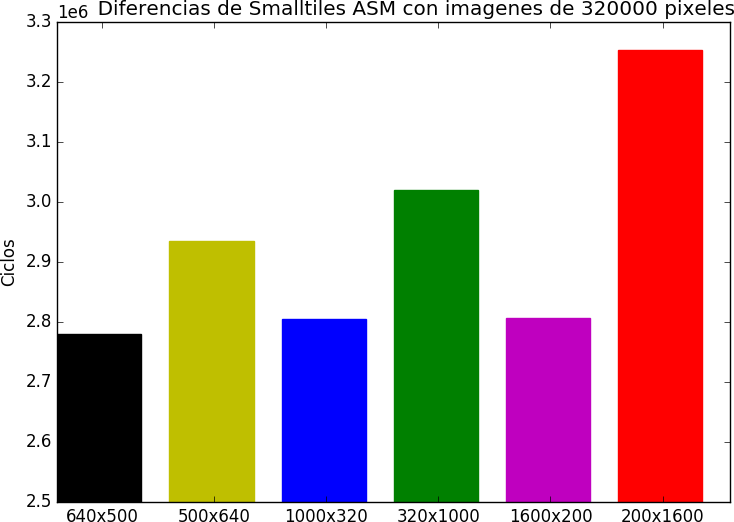
\includegraphics[width = 15 cm, height = 10 cm]{imagenes/distintostamanos.png}
\caption{•}
\end{figure}
	
	A continuación adjuntamos el gráfico que compara la cantidad de ciclos que tarda en ejecutarse el filtro implementado en ASM y el implementado en C.
	\begin{figure}[h!]
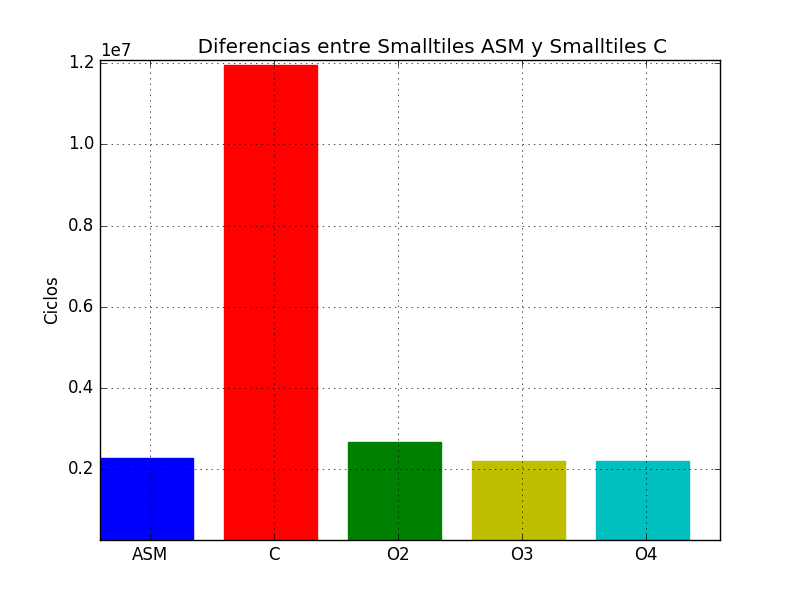
\includegraphics[width = 15 cm, height = 10 cm]{imagenes/ASMvsC.png}
\caption{•}
\end{figure}
	